\documentclass[12pt,fleqn]{article}\usepackage{../common}
\begin{document}
Ders 19

Eslenik Gradyan (Conjugate Gradient) Yontemi 

Arnoldi metotu Gram-Schmidt'e tam olmsa da benzeyen bir yontemdir ve bir
ortogonal baz ortaya cikartir. Bu baz, Krylov altuzayinin bazidir, ki bu
altuzaydaki her yeni baz vektor, $e$'nin baska bir ustu alinip carpilarak
elde edilir. Fakat bu pek iyi bir baz degildir, bazlarin ortogonalize
edilmesi gerekir, ve Arnoldi'nin yaptigi budur. 

Arnoldi-Lanczos yontemi ozdegerler (eigenvalue) bulmak icin de kullanilir.

\[ AQ = QH \]

esitligindeki $H$ matrisinin alt-matrisine bakilirsa, aranilan ozdegerler
buradan okunabilir. Bu alt-matris simetrik ve ust kosegendir.
(upperdiagonal). 

\[ H = Q^{-1}AQ \]

formulunde $H,A$ matrisleri birbirine benzerdir (similar) ve benzer
matrislerin ozdegerleri aynidir. 

Bu kavramlardan soyle bir bahsetmek istedim, belki gunun birinde cok buyuk
bir matrisin ozdegerlerini bulmak istersiniz, aklinizda olsun. Yazilim
\verb!arpack! bunun icin kullanilabiliyor. Bahsi yaptik bir diger sebep
lineer cebirin yarisi lineer sistemlerse, diger yarisi ozdeger
problemleridir denebilir. Buraya gelmisken ustteki ozdeger yonteminden
bahsetmemek olmazdi. 

Konumuza donelim. 

$A$ pozitif kesin ve simetrik olmali. Eger degilse birazdan gosgterecegimiz
formulleri kullanmak biraz riskli olur, isleyebilirler ama garanti olmaz. 

$r_K = b - Ax_k $, $K_k$'ye ortogonal, $x_k \in \mathscr{K}_K$. 

Demek ki $x_k$'yi ozyineli olarak yaratabiliriz, ve her adimda sadece $A$
ile carpmamiz gerekir. Ustteki formulde $A$ ile carpim olduguna gore, $r_K$
bir sonraki uzay $k+1$ icinde olacaktir. Arnoldi'den biliyoruz ki $q_{k+1}$
ayni uzay icindedir. O zaman 

$r_k$, $q_{k+1}$'in bir katidir. Yani $r$ ile gosterilen ``artiklar
(residuals)'' birbirine ortogonal. Yani 

\[ r_i^Tr_k = 0, \ i < k \]

Artiklarin birbirine ortogonal olmasinin sebebi iclerinde $A$ olmasi. 

Baslangic degerleri

\[ d_0 = b \]

\[ x_0 = 0 \]

\[ r_0 = b - Ax_0  = b\]

Simetrik Pozitif Kesin $A$ Icin Eslenik Gradyan Metodu

\begin{lstlisting}[language=Matlab,mathescape,numbers=left,xleftmargin=3.0ex]
$\alpha_k = r_{k-1}^T r_{k-1} / d_{k-1}^T A d_{k-1}$
$\alpha_k = \alpha_{k-1} + \alpha_k d_{k-1}$
$r_k = r_{k-1} - \alpha_k Ad_{k-1}$
$\beta_k = r_k^Tr_k / r_{k-1}^Tr_{k-1}$
$d_k = r_k + \beta_k d_{k-1}$
\end{lstlisting}

$d$ ``arama yonudur'', optimizasyon ilerlerken gidecegimiz
istikamettir. 2. adimda guncellemeyi yapiyorum. Peki bir sonraki yonum ne
olmali? 

Her Dongude:

- $Ad$ carpimini goruyoruz, cunku $A$ ile carpim bize yeni Krylov altuzayini
veriyor.\\
- 2 icsel carpim \\
- 2 ya da 3 vektor guncellemesi

Peki $k$ adim sonra hata $||e_k||$ nedir ve ilk bastaki hata $||e_0||$ ile
baglantisi nedir? 

\[ ||e_k|| \le 2  \bigg(
\frac{ \sqrt{ \lambda_{maks} - \lambda_{min}}}
{\lambda_{maks} + \lambda_{min}}
\bigg)^k||e_0||
\]

Hala bir kelimeye aciklik getirmedik; gradyan. Niye bir ``gradyan''
kelimesi kullaniyoruz, neyin gradyanindan bahsediyoruz, bu teknik icin
gradyanlar ne anlama geliyor?

Lineer problemlerde $Ax = b$ esitligi vardir ve bu esitlik enerjinin
gradyanindan gelir. Yani 

\[ E(x) = \frac{ 1}{2}x^TAx - b^Tx \]

enerjisinin gradyanindan. Ustteki formul nereden geldik diye
dusunebilirsiniz, hep lineer sistemlerden bahsettik, ve bu sistemlerde her
sey $Ax = b$ formatina uyar. Simdi birdenbire matematigin farkli bir koluna
geciyorum sanki, ustteki formulu minimize etmeye ugrasiyorum, yani
optimizasyona giriyorum. Fakat cebirsel olarak dusunursek, 

\[ grad \ E = [\frac{\partial E}{\partial x} ]  = Ax - b \]

olacaktir. Minimumda ustteki sifir olacagina gore 

\[ Ax - b = 0 \]

\[ Ax = b \]

Yani karesel enerjinin lineer gradyani vardir, ve onun minimumu $Ax =
b$'dir. 
Bu demektir ki lineer denklemi cozmek ve enerjiyi minimize etmek
aslinda ayni seydir! Minimum kelimesini kullanabiliyorum bu arada, cunku
$A$'nin pozitif kesin oldugunu biliyorum. 

Minimize islemi nasil yapilir? Diyelim ki alttaki gibi bir $E(x)$'im var,
kap seklinin herhangi bir noktasindayim, ve asagi inmem lazim. En fazla
artis gradyan $g$ ise, dibe inmek icin $-g$ yonunde gidebilirim. 

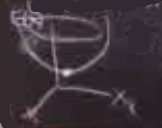
\includegraphics[height=2cm]{19_1.png}

Bu yon dogal bir yondur, ilk akla gelen fikirdir ve mantiklidir. Fakat en
iyi yon degildir. Simdi minimizasyon cozumu olarak eslenik gradyan
acisindan bakiyoruz olaya, isin gradyan tarafi da boylelikle acikliga
kavusacak. 

Negatif gradyanin ayni zamanda artigin da (residual) negatif
yonudur. Artigin yonunde hareket etmek iyi midir? Negatif gradyani takip
etmenin bir diger ismi ``en dik inis (steepest descent)''tir. Fakat,
baslangic noktasina gore bu degisir ama, cok fazla inis cikis ta
yasanabilir.

$r$'ler hesapsal bilimde cok aranan bir ozellige sahip degildir,
ortogonallik. Bir sekilde ortogonallik her zaman dogru yonde hareket
ettigimizin garantisidir. Gidilmesi gereken dogru yon, ustteki kodda
5. satirda hesaplanan yondur. Bu yone ``$A$-ortogonal'' denir. 

Bir resimle gostermek gerekirse, alta bakalim, soldaki en dik inis, sagdaki
eslenik gradyan. Enerji fonksiyonunu kesit seviyesinden (level set), cevrit
(contour) olarak gosteriyoruz, her cevrit bir enerji seviyesine tekabul
edecek, mesela en distaki cevrit 5, bir icerideki 4 olabilir, ve en
ortadaki nokta tam sifir olabilir, cunku en dusuktur. 

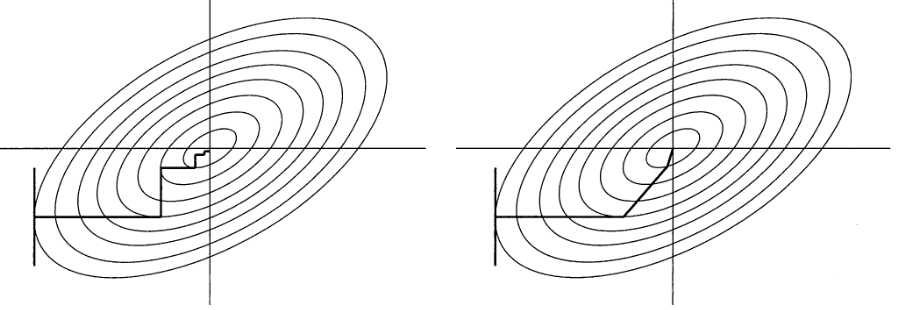
\includegraphics[height=4cm]{19_2.png}

Her iki teknigin gidisati resimde gorulmektedir. 

[gerisi atlandi]

\end{document}
